% \iffalse meta-comment
%<*internal>
\iffalse
%</internal>
%<*readme>
----------------------------------------------------------------
tikzmark --- remembering absolute positioning with TikZ
E-mail: loopspace@mathforge.org
Released under the LaTeX Project Public License v1.3c or later
See http://www.latex-project.org/lppl.txt
----------------------------------------------------------------

The tikzmark package defines a command to "remember" a position
on a page for later (or earlier) use, primarily (but not
exclusively) with TikZ.
%</readme>
%<*internal>
\fi
\def\nameofplainTeX{plain}
\ifx\fmtname\nameofplainTeX\else
  \expandafter\begingroup
\fi
%</internal>
%<*install>
\input docstrip.tex
\keepsilent
\askforoverwritefalse
\preamble
----------------------------------------------------------------
tikzmark --- remembering absolute positioning with TikZ.
E-mail: loopspace@mathforge.org
Released under the LaTeX Project Public License v1.3c or later
See http://www.latex-project.org/lppl.txt
----------------------------------------------------------------

\endpreamble
\postamble

Copyright (C) 2011-2018 by Andrew Stacey <loopspace@mathforge.org>

This work may be distributed and/or modified under the
conditions of the LaTeX Project Public License (LPPL), either
version 1.3c of this license or (at your option) any later
version.  The latest version of this license is in the file:

http://www.latex-project.org/lppl.txt

This work is "maintained" (as per LPPL maintenance status) by
Andrew Stacey.

This work consists of the file  tikzmark.dtx
and the derived files           tikzmark.ins,
                                tikzmark.pdf,
                                tikzlibrarytikzmark.code.tex, and
                                tikzmarklibrarylistings.code.tex

\endpostamble
\usedir{tex/latex/tikzmark}
\generate{
  \file{tikzlibrarytikzmark.code.tex}{\from{\jobname.dtx}{tikzlibrary}}
}
\generate{
  \file{tikzmarklibrarylistings.code.tex}{\from{\jobname.dtx}{listings}}
}
%\generate{
% \file{tikzmarklibraryhighlight.code.tex}{\from{\jobname.dtx}{highlight}}
%}
%</install>
%<install>\endbatchfile
%<*internal>
\usedir{source/latex/tikzmark}
\generate{
  \file{\jobname.ins}{\from{\jobname.dtx}{install}}
}
\nopreamble\nopostamble
\usedir{doc/latex/demopkg}
\generate{
  \file{README.txt}{\from{\jobname.dtx}{readme}}
}
\ifx\fmtname\nameofplainTeX
  \expandafter\endbatchfile
\else
  \expandafter\endgroup
\fi
%</internal>
%<*driver>
\documentclass{ltxdoc}
\usepackage[T1]{fontenc}
\usepackage{lmodern}
\usepackage{amsmath}
%\usepackage{morefloats}
\usepackage{listings}
\usepackage{tikz}
\usetikzlibrary{fit,arrows,tikzmark,shadows,decorations.pathreplacing,calc}
\usetikzmarklibrary{listings}

%\usepackage[numbered]{hypdoc}
\definecolor{lstbgcolor}{rgb}{0.9,0.9,0.9} 
 
\usepackage{listings}
\lstloadlanguages{[LaTeX]TeX}
\lstset{gobble=2,breakatwhitespace=true,breaklines=true,language=TeX}
 
\usepackage{fancyvrb}

\usepackage[hyperindex=false]{hyperref}
                                
\newenvironment{example}
  {\VerbatimEnvironment
   \begin{VerbatimOut}[gobble=2]{example.out}}
  {\end{VerbatimOut}
   \begin{center}
%   \setlength{\parindent}{0pt}
   \fbox{\begin{minipage}{.9\linewidth}
     \lstset{breakatwhitespace=true,breaklines=true,language=TeX,basicstyle=\small}
     \lstinputlisting[]{example.out}
   \end{minipage}}

   \fbox{\begin{minipage}{.9\linewidth}
     \input{example.out}
   \end{minipage}}
\end{center}
}

\newenvironment{justexample}
  {\VerbatimEnvironment
   \begin{VerbatimOut}[gobble=2]{example.out}}
  {\end{VerbatimOut}
   \begin{center}
%   \setlength{\parindent}{0pt}
   \fbox{\begin{minipage}{.9\linewidth}
     \lstset{breakatwhitespace=true,breaklines=true,language=TeX,basicstyle=\small}
     \lstinputlisting[]{example.out}
   \end{minipage}}
\end{center}
}

  \newcommand\balloon[4]{%
    \pgfmathtruncatemacro\firstline{%
      #3-1
    }%
    \iftikzmark{line-#2-\firstline-start}{%
      \iftikzmark{line-#2-#3-first}{%
        \xdef\blines{({pic cs:line-#2-\firstline-start} -| {pic cs:line-#2-#3-first})}%
      }{%
        \iftikzmark{line-#2-#3-start}{%
          \xdef\blines{({pic cs:line-#2-\firstline-start} -| {pic cs:line-#2-#3-start})}%
        }{%
          \xdef\blines{(pic cs:line-#2-\firstline-start)}%
        }%
      }%
    }{%
      \xdef\blines{}%
    }%
    \foreach \k in {#3,...,#4} {%
      \iftikzmark{line-#2-\k-first}{%
        \xdef\blines{\blines (pic cs:line-#2-\k-first) }
      }{}
      \iftikzmark{line-#2-\k-end}{%
        \xdef\blines{\blines (pic cs:line-#2-\k-end) }
      }{}
    }%
    \ifx\blines\empty
    \else
    \edef\temp{\noexpand\tikz[remember         picture,overlay]{\noexpand\node[fit={\blines},balloon] (#1) {}}}%
    \temp
    \fi
  }
  \tikzset{
    line/.style={
      draw,
      rounded corners=3pt,
      -latex
    },
    balloon/.style={
      draw,
      fill=blue!20,
      opacity=0.4,
      inner sep=4pt,
      rounded corners=2pt
    },
    comment/.style={
      draw,
      fill=blue!70,
      text=white,
      text width=3cm,
      minimum height=1cm,
      rounded corners,
      drop shadow,
      align=left,
      font=\scriptsize
    },
  }

\DisableCrossrefs
% \CodelineIndex
\RecordChanges
\begin{document}
  \DocInput{\jobname.dtx}
\end{document}
%</driver>
% \fi
%
% \CheckSum{1138}
%
% \CharacterTable
%  {Upper-case    \A\B\C\D\E\F\G\H\I\J\K\L\M\N\O\P\Q\R\S\T\U\V\W\X\Y\Z
%   Lower-case    \a\b\c\d\e\f\g\h\i\j\k\l\m\n\o\p\q\r\s\t\u\v\w\x\y\z
%   Digits        \0\1\2\3\4\5\6\7\8\9
%   Exclamation   \!     Double quote  \"     Hash (number) \#
%   Dollar        \$     Percent       \%     Ampersand     \&
%   Acute accent  \'     Left paren    \(     Right paren   \)
%   Asterisk      \*     Plus          \+     Comma         \,
%   Minus         \-     Point         \.     Solidus       \/
%   Colon         \:     Semicolon     \;     Less than     \<
%   Equals        \=     Greater than  \>     Question mark \?
%   Commercial at \@     Left bracket  \[     Backslash     \\
%   Right bracket \]     Circumflex    \^     Underscore    \_
%   Grave accent  \`     Left brace    \{     Vertical bar  \|
%   Right brace   \}     Tilde         \~}
%
%
% \changes{1.0}{2012/11/08}{Converted to DTX file}
% \changes{1.1}{2013/04/22}{Fix bug relating to active semi-colon}
% \changes{1.2}{2016/04/07}{Tikzmark works inside tikzpicture, added easy suffix and prefix for tikzmarks}
% \changes{1.3}{2017/06/01}{Tikzmark no longer uses semi-colon (too many issues with catcodes) and fix for beamer-awareness}
% \changes{1.4}{2017/10/29}{Bug fixes: spurious characters in aux file, tikzmark prefix/suffix ignored in iftikzmark test}
% \changes{1.5}{2018/09/09}{Reintroduced the original command (now as tikzmarknode) with a mathchoice hack for different math modes}
% \changes{1.6}{2018/10/18}{Added the ability to save node information between runs and between TeX documents}
% \changes{1.7}{2019/05/07}{Added conditions to test if a tikzmark is on a particular page}
%
% \DoNotIndex{\newcommand,\newenvironment}
%
% \providecommand*{\url}{\texttt}
% \title{The \textsf{tikzmark} package}
% \author{Andrew Stacey \\ \url{loopspace@mathforge.org}}
% \date{v1.7~from 2019/05/07}
%
%
% \maketitle
%
% 
% \section{Introduction}
%
% The \Verb+\tikzmark+ macro burst onto the scene in a blaze of glory on \href{http://tex.stackexchange.com}{TeX-SX}.
% Since then, it has proved embarrassingly (to its original author) popular.
% The idea behind it is extremely simple: that the machinery underneath TikZ provides a way to ``mark'' a point on a page for further use.
% This functionality is already provided by several other packages.
% The point of this one is that as TikZ can provide this feature, if already loading TikZ then it makes sense to use the TikZ version than another version.
% Moreover, if the goal is to use these marks with some TikZ code then this version is already set up for that purpose (not that it would be exactly difficult to add this to any of the other implementations).
%
% \section{Use}
%
% Using the \Verb+\tikzmark+ is extremely simple.
% You need to load the \Verb+tikz+ package and then load \Verb+tikzmark+ as a \Verb+tikzlibrary+.
% Thus in your preamble you should have something like:
%
% \begin{lstlisting}
% \usepackage{tikz}
% \usetikzlibrary{tikzmark}
% \end{lstlisting}
%
% In your document, you can now type \Verb+\tikzmark{<name>}+ at a point that you want to remember.
% This will save a mark with name \Verb+<name>+ for use later (or earlier).
% To use it in a \Verb+\tikz+ or \Verb+tikzpicture+, simply use the \Verb+pic+ coordinate system:
%
% \begin{lstlisting}
% \tikz[remember picture] \draw[overlay] (0,0) -- (pic cs:<name>);
% \end{lstlisting}
%
% There are two important points to note:
%
% \begin{enumerate}
% \item The enveloping \Verb+\tikz+ or \Verb+tikzpicture+ must have the key \Verb+remember picture+ set.
%
% This is because of how TikZ coordinates work.
% The coordinates inside a TikZ picture are relative to its origin, so that origin can move around on the page and not affect the internals of the picture.
% To use a point outside the picture, therefore, the current picture not only has to know where that point is on the page it also has to know where it itself is on the page.
% Hence the \Verb+remember picture+ key must be set.
% \item The drawing command must have the \Verb+overlay+ key set (or be in a scope or picture where it is set).
% 
% This is to keep the bounding box of the current picture under control.
% Otherwise, it would grow to encompass the remembered point as well as the current picture.
% (This isn't necessary if the remembered point is inside the current picture.)
% \end{enumerate}
%
% 
%
% \section{History}
%
% I wrote the original \Verb+\tikzmark+ macro in 2009 for use in lecture slides prepared with the \Verb+beamer+ package.
% Its original definition was:
%
% \begin{lstlisting}
% \newcommand{\tikzmark}[1]{\tikz[overlay,remember picture] \node (#1) {};}
% \end{lstlisting}
%
% Its first use was in the (inelegant) code:
%
% \begin{lstlisting}
% \begin{frame}
% \frametitle{Structure of Continuous Functions}
%
% \begin{tikzpicture}[overlay, remember picture]
% \useasboundingbox (0,0);
% \draw<2-|trans: 0|handout: 0>[red,->] (bsp) .. controls +(-1,-1) and ($(cnvs.north)+(1,1)$) .. ($(cnvs.north)+(0,1)$) .. controls ($(cnvs.north)+(-1,1)$) and +(-1,0) .. (cnvs.north);
% \draw<3-|trans: 0|handout: 0>[green!50!black,->] (cplt) .. controls +(-1,-1) and +(-1,0) .. (mcplt.north);
% \draw<4-|trans: 0|handout: 0>[blue,->] (norm) .. controls +(-1,-.5) and ($(nvs.north)+(0,1.5)$) .. ($(nvs.north)+(0,1.5)$) .. controls ($(nvs.north)+(-1.5,1.5)$) and +(-1.5,0) .. (nvs.north);
% \draw<5-|trans: 0|handout: 0>[purple,->] (vector) .. controls +(-1,-1) and ($(vsp.north)+(2,2)$) .. ($(vsp.north)+(0,2)$) .. controls ($(vsp.north)+(-2,2)$) and +(-2,0) .. (vsp.north);
% \end{tikzpicture}
%
% \begin{theorem}
% \centering
% \(\big(C([0,1],\R),d_\infty\big)\) \\
% is a \\
% \alert{Banach\tikzmark{bsp} space}
% \end{theorem}
%
% \pause
% \bigskip
%
% \begin{itemize}
% \item[\tikzmark{cnvs}] {\color<.(2)->{green!50!black}Comp\tikzmark{cplt}lete} {\color<.(3)->{blue}nor\tikzmark{norm}med} {\color<.(4)->{purple}vector\tikzmark{vector} space}.
%
% \bigskip
% \bigskip
% \pause
%
% \begin{itemize}[<+->]
% \item[\tikzmark{mcplt}] {\color{green!50!black}Cauchy sequences converge.}
% \medskip
% \item[\tikzmark{nvs}] {\color{blue}Metric from a norm.}
% \medskip
% \item[\tikzmark{vsp}] {\color{purple}Functions behave like vectors.}
% \end{itemize}
% \end{itemize}
%
% \end{frame}
% \end{lstlisting}
%
% This produced, on the final slide, Figure~\ref{fig:tikzmarkex}.
%
% \begin{figure}
% \centering
% \IfFileExists{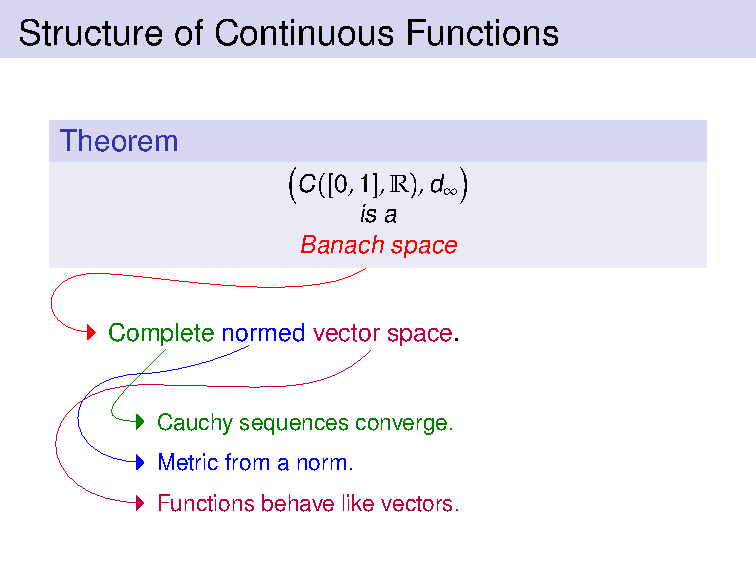
\includegraphics{tikzmarkExample}}{}
% \caption{First use of tikzmark}
% \label{fig:tikzmarkex}
% \end{figure}
%
% Its first appearance on \href{http://tex.stackexchange.com}{TeX-SX} was in an \href{http://tex.stackexchange.com/a/316/86}{answer} to a question about how to put overlapping braces on a mathematical text.
% This was in July 2010.
% The opening statement of the answer was not overly encouraging: ``This may not be the best solution\dots''.
% And for a macro that would go on to become quite ubiquitous, its initial appearance only garnered it 2 votes.
%
% However, it started out in life as a useful macro for me and as such I found more uses for it in my own code and thus more opportunity for using it to answer questions on TeX-SX.
% The one that seems to have been where it got noticed came in \href{http://tex.stackexchange.com/a/1570/86}{August 2010}, again about putting braces in text but in a more complicated fashion.
% From this answer, it got picked up, picked over, and picked apart.
% A common use was in highlighting or adding marks to text.
%
% Gradually, as it got used, it developed.
% A major revision dates from an answer given in \href{http://tex.stackexchange.com/a/50054/86}{March 2012} where the question was actually about \Verb+\tikzmark+.
% This version added two important features: a TikZ coordinate system for referencing saved marks directly and the ability to refer to marks earlier in the document than they are defined (the mechanism for remembering points uses the \Verb+aux+ file anyway so this was more about exposing the information earlier than anything complicated).
% Then in October 2012 there was a  \href{http://tex.stackexchange.com/q/79121/86}{question} where it would have been useful to remember which page the mark was on and a \href{http://tex.stackexchange.com/q/79762/86}{question} where for some reason using the \Verb+\tikz+ macro didn't work so the \Verb+\pgfmark+ macro was introduced.
%
% By this point, the \Verb+\tikzmark+ command had morphed considerably from its original definition.
% Experience has shown that on the TeX-SX site it has continued to be used in its original form as well as its current form.
% I've therefore taken the decision to reintroduce a form of the original command, now called \Verb+\tikzmarknode+.
% It goes beyond the original version in that it uses some \Verb+\mathchoice+ trickery (inspired by \href{https://tex.stackexchange.com/a/122419/86}{this answer} from Heiko Oberdiek) to hopefully correctly choose the correct math style.
%
% The original reason for not using nodes inside \Verb+\tikzmark+ was to be able to use the information from a \Verb+\tikzmark+ before the point where it was defined (via information saved into the \Verb+aux+ file).
% Thanks to a \href{https://tex.stackexchange.com/a/415862/86}{question on TeX-SX} about saving node information, I've developed code that solves that issue with nodes.
% As it fits in the general concept of this package, I've added that code to the \Verb+\tikzmark+ package.
%
% \section{Usage}
%
% This package defines the following commands and usable stuff.
%
% \begin{enumerate}
% \item \Verb+\tikzmark+\oarg{drawing command}\marg{name}
%
% The mandatory argument is the name of the mark to be used to refer back to this point later.
%
% The \Verb+\tikzmark+ command can take an optional parameter which is some drawing command that can be put in a \Verb+\tikz ... ;+ command.
% This drawing command can be used to place a node or something similar at the marked point, or to set some \Verb+\tikzset+ keys.
% Sometimes this can be useful.
% Note, though, that if this is used to define an offset coordinate then this will only be available in the document \emph{after} the \Verb+\tikzmark+ command, even on later runs.
%
% If the \Verb+beamer+ class is loaded then this command is made overlay-aware.
%
% \item \Verb+\tikzmark+\marg{name}\marg{coordinate}
%
% v1.2 of the \Verb+tikzmark+ package introduced a new variant of \Verb+\tikzmark+ which works inside a \Verb+tikzpicture+.
% One feature of \Verb+\tikzmark+ which isn't part of TikZ's normal coordinate remembering system is the ability to use a \Verb+\tikzmark+ coordinate before it is defined (due to the use of the \Verb+aux+ file).
% This is potentially useful to have inside a \Verb+tikzpicture+ and so it is now possible to use \Verb+\tikzmark+ inside a \Verb+tikzpicture+.
% The syntax is slightly different as we need to specify the coordinates of a point to remember.
%
% This was inspired by the question \href{http://tex.stackexchange.com/q/295903/86}{Refer to a node in tikz that will be defined ``in the future'' (two passes)?} on TeX-SX.
%
% \item \Verb+\pgfmark+\marg{name}
%
% This is a more basic form of the \Verb+\tikzmark+ which doesn't use any of the \Verb+\tikz+ overhead.
% One advantage of this command is that it doesn't create an \Verb+hbox+.
% It does, however, insert a \Verb+whatsit+ into the stream so it will, for example, stop two vertical spaces either side of it being merged.
% This can't be avoided.
% 
% If the \Verb+beamer+ class is loaded then this command is made overlay-aware.
%
% \item \Verb+\iftikzmark+\marg{name}\marg{true code}\marg{false code}
%
% This is a conditional to test if a particular mark is available.
% It executes \Verb+true code+ if it is and \Verb+false code+ if not.
%
% \item \Verb+\iftikzmarkexists+\marg{name}
%
% This is a conditional to test if a particular mark is available which works with the lower level \TeX\ \Verb+\else+ and \Verb+\fi+.
%
% \item \Verb+\iftikzmarkoncurrentpage+\marg{name}
%
% This is a conditional to test if a particular mark is on the current page; it works with the lower level \TeX\ \Verb+\else+ and \Verb+\fi+.
%
% \item \Verb+\iftikzmarkonpage+\marg{name}\marg{page}
%
% This is a conditional to test if a particular mark is on a given page; it works with the lower level \TeX\ \Verb+\else+ and \Verb+\fi+.
%
% \item \Verb+\tikzmarknode+\oarg{options}\marg{name}\marg{contents}
%
% This is a reincarnation of the original \Verb+\tikzmark+ command which places its contents inside a \Verb+\tikz+ node.  It also defines a \Verb+tikzmark+ with the same name.  Using a sneaky trick with \Verb+\mathchoice+, it works inside a math environment.  The spacing either side might not be quite right as although it detects the math style it doesn't got beyond that. The \Verb+options+ are passed to the node.
%
% Two styles are attempted, one on the surrounding picture and one on the node, which are:
%
% \begin{itemize}
% \item \Verb+every tikzmarknode picture+
% \item \Verb+every tikzmarknode+
% \end{itemize}
%
% To refer to the \emph{node}, use usual TikZ coordinates.
% To refer to the underlying \emph{tikzmark}, use the special tikzmark coordinates (see below).
%
% \item \Verb+(pic cs:<name>)+ or \Verb+(pic cs:<name>,<coordinate>)+
%
% This is the method for referring to a position remembered by \Verb+\tikzmark+ (or \Verb+\pgfmark+) as a coordinate in a \Verb+tikzpicture+ environment (or \Verb+\tikz+ command).
% If the extra \Verb+coordinate+ is specified then this is used in case the mark \Verb+name+ has not yet been defined (this can be useful for defining code that does something sensible on the first run).
%
% \item \Verb+/tikz/save picture id=<name>+
%
% This is the TikZ key that is used by \Verb+\tikzmark+ to actually save the connection between the name and the picture coordinate.
% It can be used on an arbitrary picture to save its origin as a tikzmark.
%
% \item \Verb+/tikz/if picture id=#1#2#3+
%
% This is a key equivalent of the \Verb+\iftikzmark+ command.
%
% \item \Verb+/tikz/if tikzmark on current page=#1#2#3+
%
% This is a key equivalent of the \Verb+\iftikzmarkoncurrentpage+ command.
% If true, the keys in \Verb+#2+ are executed, otherwise the keys in \Verb+#3+.
%
% \item \Verb+/tikz/if tikzmark on page=#1#2#3#4+
%
% This is a key equivalent of the \Verb+\iftikzmarkonpage+ command.
%
% \item \Verb+/tikz/next page+, \Verb+/tikz/next page vector+
%
% It is possible to refer to a mark on a different page to the current page.
% When this is done, the mark is offset by a vector stored in the key \Verb+/tikz/next page vector+.
% The key \Verb+/tikz/next page+ can be used to set this to certain standard vectors by specifying where the ``next page'' is considered as lying corresponding to the current page.
% Possible values are (by default) \Verb+above+, \Verb+below+, \Verb+left+, \Verb+right+, and \Verb+ignore+.
% (The last one sets the vector to the zero vector.)
%
% \item \Verb+/tikz/tikzmark prefix=<prefix>+  and \Verb+/tikz/tikzmark suffix=<suffix>+
%
% These keys allow for the automatic addition of a prefix and/or suffix to each \Verb+\tikzmark+ name.
% The prefix and suffix are added both at time of definition and of use, so providing one is in the same scope there is no difference in at the user level when using prefixes and suffixes.
% What it can be useful for is to make the \Verb+\tikzmark+ names unique.
% In particular, if the \Verb+beamer+ class is loaded then an automatic suffix is added corresponding to the overlay.
% This means that if a slide consists of several overlays with \Verb+\tikzmark+s on them, and the positions of the \Verb+\tikzmark+s move then the resulting pictures should look right. 
% Without the automatic suffix, only the final positions of the marks would be used throughout.
%
% This was inspired by the question \href{http://tex.stackexchange.com/q/302517/86}{using tikzmark subnode with overlays beamer} on TeX-SX.
%
% \item \Verb+\subnode[options]{name}{content}+
%
% This produces a pseudo-node named \Verb+name+ around the \Verb+content+.
% The design purpose of this is to create a ``subnode'' inside a TikZ node.
% As far as TikZ is concerned, the contents of a node is just a box.
% It therefore does not know anything about it beyond its external size and so cannot easily determine the coordinates of pieces inside.
% The \Verb+\subnode+ command boxes its contents and saves the position of that box and its dimensions.
% This information is stored in the same way that PGF stores the necessary information about a node.
% It is therefore possible to use ordinary node syntax (within a \Verb+tikzpicture+) to access this information.
% Thus after \Verb+\node {a \subnode{a}{sub} node};+ it is possible to use \Verb+a+ as a node.
% The \Verb+options+ are passed to the node construction mechanism, but note that the only sensible options are those that affect the size and shape of the node: drawing options are ignored (except in so far as they affect the size -- as an example, \Verb+line width+ affects the node size).
%
% There are two important points to make about this.
% The first is that, as with all the \Verb+tikzmark+ macros, the information is always one compilation old.
% The second is that the pseudo-node is purely about coordinates: the  path information is not used and the contents are not moved.
% This is partly for reasons of implementation: the pseudo-node is constructed when TikZ is not in ``picture mode''.
% But also interleaving the background path of the pseudo-node and any containing node would be problematic and so is best left to the user.
%
% The simplest way to turn a pseudo-node into a more normal node is to use the \Verb+fit+ library.
% Using the above example, \Verb+\node[fit=(a),draw,inner sep=0pt] {};+ would draw a rectangle around the word \Verb+sub+ of exactly the same size as would appear had a normal node been created.
%
% Using a sneaky trick with \Verb+\mathchoice+, \Verb+subnode+ works inside a math environment.  The spacing either side might not be quite right as although it detects the math style it doesn't got beyond that.
%
% \item \emph{Node saving}
%
% The node saving system takes the information stored about a node and saves it for later use.
% That later use can be in the same document, in which case it should be saved just to the memory of the current TeX process, or it can be used earlier in the same document or another document altogether (in particular, if the nodes are defined in a \Verb+tikzpicture+ that has been externalised, this can be used to import the node information into the main file) in which cases the node data is saved to a file.
%
% When working with files, nodes are saved and restored in bulk.
% When working in memory, nodes are saved and restored in named lists.
% Nodes are not actually saved until the end of the tikzpicture in which they are defined, meaning that if saving to memory then all the nodes in a tikzpicture will belong to the same list.
%
% The keys for working with saving and restoring nodes are as follows.
%
% \begin{itemize}
% \item \Verb+save node+
%
% This is the key to put on a node that is to be saved.
%
% \item \Verb+set node group=<name>+
%
% Nodes are grouped together into a list that can be saved either to a file or for use later on in the document.
% This sets the name for the current group.
%
% \item \Verb+restore nodes from list=<name>+
%
% This restores the node information from the named list to the current \Verb+tikzpicture+.
% This is required both for when the node information comes from a file or from earlier in the same document.
%
% \item \Verb+save nodes to file+
%
% This is a \Verb+true/false+ key which determines whether to save the node information to a file.
%
% \item \Verb+set saved nodes file name=<name>+
%
% This sets the file name for the saved nodes (the extension will be \Verb+.nodes+.
% The default is to use the current \TeX\ filename.
% This is set globally, and once the file is opened then changing the name will have no effect.
% (The file is not opened until it is actually needed to avoid creating empty files unnecessarily.)
%
% \item \Verb+restore nodes from file=<name>+
%
% This loads the node information from the file into the current document.
%
% The \Verb+<name>+ can have the syntax \Verb+[options]{name}+, where \Verb+options+ can be used to influence how the nodes are restored.
% The key \Verb+transform saved nodes+ (see below) can be given here.
% Another useful key is the \Verb+name prefix+ key which is applied to all restored nodes.
%
% \item \Verb+transform saved nodes+
%
% A particular use-case for restoring saved nodes is to safely include one \Verb+tikzpicture+ inside another by creating an image out of the inner picture and including it back in as a picture inside a node.
% In that situation, restoring the nodes from the inner picture can make it possible to refer to coordinates from the inner picture to the outer one.
% If there is a transformation in place on the containing node, this key applies that transformation to all the nodes in the inner picture.
%
% \end{itemize}
% \end{enumerate}
%
% \section{Examples and Extras}
%
% The \Verb+\tikzmark+ command has been used in numerous answers on \href{http://tex.stackexchange.com}{TeX-SX}.
% The plan is to gather some of these into extra libraries which can be loaded via \Verb+\usetikzmarklibrary+.
%
% At present, this is the code listings library (which works with the \Verb+listings+ package).
% One that is in development (as it has featured much on the TeX-SX website) is highlighting, however this is not so straightforward to implement so is still under development.
%
% \subsection{Basic Examples}
%
% A simple example of the \Verb+\tikzmark+ macro is the following.
%
% \begin{example}
% \[
%  \tikzmark{a} e^{i \pi/2} = i
% \]
%
% This\tikz[remember picture,overlay,baseline=0pt] \draw[->] (0,1em) to[bend left] ([shift={(-1ex,1ex)}]pic cs:a); is an important equation.
% \end{example}
%
% \begin{example}
% \begin{itemize}
% \item A first item,\tikzmark{b}
% \item A second item,\tikzmark{c}
% \item A third item.\tikzmark{d}
% \end{itemize}
% \begin{tikzpicture}[remember picture,overlay]
% \draw[decorate,decoration={brace}] ({pic cs:c} |- {pic cs:b}) +(0,1em) -- node[right,inner sep=1em] {some items} ({pic cs:c} |- {pic cs:d});
% \end{tikzpicture}
% \end{example}
%
% \begin{example}
% \begin{tikzpicture}[remember picture]
% \node (a) at (0,0) {This has a \subnode{sub}{subnode} in it};
% \draw[->] (0,-1) to[bend right] (sub);
% \end{tikzpicture}
% \end{example}
%
% An example using \Verb+\tikzmark+ inside a \Verb+tikzpicture+
%
% \begin{example}
% \tikzset{tikzmark prefix=ex3-}
% \begin{tikzpicture}[remember picture,overlay]
% \draw[->,line width=1mm,cyan] (pic cs:a) to[bend left] (pic cs:b);
% \end{tikzpicture}
%
% By placing the \tikzmark{a}code before the marks, the arrow goes under the subsequent text and picture.
%
% \begin{tikzpicture}
% \filldraw[fill=gray] (0,0) circle[radius=1cm];
% \tikzmark{b}{(-1,-1)}
% \end{tikzpicture}
% \end{example}
%
% The \Verb+\tikmarknode+ puts a node around some text, which can be referred to later, and adds a \Verb+\tikzmark+ at its origin.
%
% \begin{example}
% Putting a node around \tikzmarknode{txt}{some text} means we can connect text together, including in maths:
% \[
% \tikzmarknode{a}{\sum_{k=1}^n} k^{\tikzmarknode{b}{2}}
% \]
%
% \begin{tikzpicture}[remember picture,overlay]
% \draw[->] (txt) -- (a);
% \draw[->] (a.south) to[out=-90,in=-45] (b.south east);
% \end{tikzpicture}
% \end{example}
%
% The syntax for saving node data is illustrated by the following example.
%
% File \Verb+firstpicture.tex+:
%
% \begin{justexample}
% \documentclass[tikz,border=10pt]{standalone}
% \usetikzlibrary{tikzmark,shapes.geometric}
% \begin{document}
% \begin{tikzpicture}[save nodes to file]
% \node[draw,rotate=-30,save node](1) at (-2,0) {1};
% \draw[->] (0,0) -- (1);
% \node[draw,ellipse,save node] (c) at (current bounding box.center) {};
% \end{tikzpicture}
% \end{document}
% \end{justexample}
%
% File \Verb+secondpicture.tex+:
%
% \begin{justexample}
% \documentclass[tikz,border=10pt]{standalone}
% \usetikzlibrary{tikzmark,shapes.geometric}
% \begin{document}
% \begin{tikzpicture}[save nodes to file]
% \node[draw,rotate=-70,save node] (2) at (2,0) {2};
% \draw[->] (0,0) -- (2);
% \node[draw,ellipse,save node] (c) at (current bounding box.center) {};
% \end{tikzpicture}
% \end{document}
% \end{justexample}
%
% Main file:
%
% \begin{justexample}
% \documentclass{article}
% \usepackage{tikz}
% \usetikzlibrary{tikzmark}
% 
% \begin{document}
% \begin{tikzpicture}
% 
% \node[draw,
%   rotate=30,
%   restore nodes from file={[transform saved nodes,name prefix=pic-1-]{firstpicture}}
% ] (a-1) at (-2,-3) {\includegraphics{firstpicture.pdf}};
% 
% \node[draw,
%   rotate=70,
%   restore nodes from file={[transform saved nodes,name prefix=pic-2-]{secondpicture}}
% ] (a-2) at (+2,+2) {\includegraphics{secondpicture.pdf}};
% 
% \draw[red] (pic-1-1.north west) --  (pic-1-1.north east) --  (pic-1-1.south east) --  (pic-1-1.south west) -- cycle;
% \draw[red] (pic-2-2.north west) --  (pic-2-2.north east) --  (pic-2-2.south east) --  (pic-2-2.south west) -- cycle;
% 
% \node[red] at (pic-1-1) {1};
% \node[red] at (pic-2-2) {2};
% 
% \draw (a-1) circle[radius=5pt];
% \draw (a-2) circle[radius=5pt];
% 
% \draw (pic-1-1) -- (pic-2-2);
% \end{tikzpicture}
% \end{document}
% \end{justexample}
%
% This produces:
%
% \begin{center}
% \fbox{\IfFileExists{tikzrefextnodes.pdf}{\includegraphics{tikzrefextnodes}}{}}
% \end{center}
%
% \subsection{Code Listings}
%
% If the \Verb+listings+ package has been loaded then issuing
%
% \Verb+\usetikzmarklibrary{listings}+
%
% \noindent will load in some code to add marks to \Verb+lstlisting+ environments.
% This code places a mark at three places on a line of code in a \Verb+listings+ environment.
% The marks are placed at the start of the line, the first non-whitespace character, and the end of the line (if the line is blank the latter two are not placed).
% (This has not been extensively tested, it works by adding code to various ``hooks'' that are made available by the \Verb+listings+ package; it is quite possible that the hooks chosen are both wrong and insufficient to cover all desired cases.)
%
%
% These are inspired by questions such as \href{http://tex.stackexchange.com/q/79762/86}{Marking lines in listings} and \href{http://tex.stackexchange.com/q/86309/86}{Macros for code annotations}.
%
% In more detail, the \Verb+listings+ library places lots of marks around the code.
% The marks are:
%
% \begin{itemize}
% \item \Verb+line-<name>-<number>-start+ at the start of each line.
% \item \Verb+line-<name>-<number>-end+ at the end of each line.
% \item \Verb+line-<name>-<number>-first+ at the first non-space character of the line (assuming it exists).
% \end{itemize}
%
% The line numbers \emph{should} match up with the line numbers in the code in that any initial offset is also applied.
%
% Not every mark is available on every line.
% If a line is blank, in particular, it will only have a \Verb+start+ mark.
% The following example shows this, where the red dots are the \Verb+start+, the blue are \Verb+end+, and the green are \Verb+first+.
%
% \begin{example}
% \begin{tikzpicture}[remember picture]
% \foreach \k in {0,...,7} {
% \iftikzmark{line-code-\k-start}{\fill[red,overlay] (pic cs:line-code-\k-start) circle[radius=4pt];}{\message{No start for \k}}
% \iftikzmark{line-code-\k-end}{\fill[blue,overlay] (pic cs:line-code-\k-end) circle[radius=2pt];}{\message{No end for \k}}
% \iftikzmark{line-code-\k-first}{\fill[green,overlay] (pic cs:line-code-\k-first) circle[radius=2pt];}{\message{No first for \k}}
% }
% \draw[->,overlay] (0,0) -- (pic cs:line-code-5-first);
% \draw[->,overlay] (0,0) -- (pic cs:line-code-5-start);
% \draw[->,overlay] (0,0) -- (pic cs:line-code-5-end);
% \node[above] at (0,0) {Line 5};
% \end{tikzpicture}
% 
% \begin{lstlisting}[language=c,name=code,numbers=left]
%   #include <stdio.h>
% 
%   int main(void)
%   {
%       printf("hello, world\n");
%       return 0;
%   }
% \end{lstlisting}
% \end{example}
%
% This example puts a fancy node behind certain lines of the code, computing the necessary extents.
%
% \begin{example}
% \balloon{comment}{more code}{3}{3}
% \balloon{comment}{more code}{7}{8}
% \begin{lstlisting}[language=c,name=more code,numbers=left,firstnumber=3]
%   #include <stdio.h>
%   
%   int main(void)
%   {
%       printf("hello, world\n");
%       return 0;
%   }
% \end{lstlisting}
% \end{example}
%
%
%
% \section{Acknowledgements}
%
% The \Verb+\tikzmark+ macro has been used and abused by many users of \href{http://tex.stackexchange.com}{TeX-SX}.
% Of particular note (but in no particular order) are \href{https://tex.stackexchange.com/users/4301/peter-grill}{Peter Grill}, \href{https://tex.stackexchange.com/users/3954/gonzalo-medina}{Gonzalo Medina}, \href{https://tex.stackexchange.com/users/13304/claudio-fiandrino}{Claudio Fiandrino}, \href{https://tex.stackexchange.com/users/3235/percusse}{percusse}, and \href{https://tex.stackexchange.com/users/121799/marmot}{marmot}.
% I would also like to mention \href{https://tex.stackexchange.com/users/1090/david-carlisle}{David Carlisle} whose knowledge of TikZ continues to astound us all.
% 
%
% \StopEventually{}
%
% \section{Implementation}
%
% \iffalse
%<*tikzlibrary>
% \fi
% \subsection{Main Code}
%
%
% The \Verb+save nodes+ code uses \LaTeX3.
%    \begin{macrocode}
\RequirePackage{expl3, l3keys2e, xparse}
%    \end{macrocode}
%
%    \begin{macrocode}
\tikzset{%
  remember picture with id/.style={%
    remember picture,
    overlay,
    save picture id=#1,
  },
%    \end{macrocode}
% Not totally happy with using \Verb+every picture+ here as it's too easily overwritten by the user.
% Maybe it would be better to patch \Verb+endtikzpicture+ directly.
%    \begin{macrocode}
  every picture/.append style={%
    execute at end picture={%
      \ifpgfrememberpicturepositiononpage%
      \edef\pgf@temp{%
        \noexpand\write\noexpand\pgfutil@auxout{%
          \string\savepicturepage%
          {\pgfpictureid}{\noexpand\arabic{page}}%
        }%
      }%
      \pgf@temp
      \fi%
    },
  },
%    \end{macrocode}
% The positions are already recorded in the \Verb+aux+ file, all we really need to do is provide them with better names.
%    \begin{macrocode}
  save picture id/.code={%
      \protected@write\pgfutil@auxout{}{%
      \string\savepointas%
      {\tikzmark@pp@name{#1}}{\pgfpictureid}{0pt}{0pt}}%
  },
%    \end{macrocode}
% Provides a way to test if a picture has already been saved (in particular, can avoid errors on first runs)
%    \begin{macrocode}
  if picture id/.code args={#1#2#3}{%
    \@ifundefined{save@pt@\tikzmark@pp@name{#1}}{%
      \pgfkeysalso{#3}%
    }{
      \pgfkeysalso{#2}%
    }
  },
%    \end{macrocode}
% Page handling
%    \begin{macrocode}
  next page/.is choice,
  next page vector/.initial={\pgfqpoint{0pt}{0pt}},
  next page/below/.style={%
    next page vector={\pgfqpoint{0pt}{-\the\paperheight}}%
  },
  next page/above/.style={%
    next page vector={\pgfqpoint{0pt}{\the\paperheight}}%
  },
  next page/left/.style={%
    next page vector={\pgfqpoint{-\the\paperwidth}{0pt}}%
  },
  next page/right/.style={%
    next page vector={\pgfqpoint{\the\paperwidth}{0pt}}%
  },
  next page/ignore/.style={%
    next page vector={\pgfqpoint{0pt}{0pt}}%
  },
  if tikzmark on current page/.code n args={3}{%
    \@ifundefined{save@pt@\tikzmark@pp@name{#1}}{%
      \pgfkeysalso{#3}%
    }{%
      \@ifundefined{save@pg@\csname save@pt@\tikzmark@pp@name{#1}\endcsname}{%
        \pgfkeysalso{#3}%
      }{%
        \ifnum\csname save@pg@\csname save@pt@\tikzmark@pp@name{#1}\endcsname\endcsname=\the\value{page}\relax%
        \pgfkeysalso{#2}%
        \else
        \pgfkeysalso{#3}%
        \fi
      }%
    }%
  },
  if tikzmark on page/.code n args={4}{%
    \@ifundefined{save@pt@\tikzmark@pp@name{#1}}{%
      \pgfkeysalso{#4}%
    }{%
      \@ifundefined{save@pg@\csname save@pt@\tikzmark@pp@name{#1}@label\endcsname}{%
        \pgfkeysalso{#4}%
      }{%
        \ifnum\csname save@pg@\csname save@pt@\tikzmark@pp@name{#1}\endcsname\endcsname=#2\relax%
        \pgfkeysalso{#3}%
        \else
        \pgfkeysalso{#4}%
        \fi
      }%
    }%
  },
%    \end{macrocode}
% Prefix and suffix for tikzmark names, shamelessly borrowed from the main tikz code  
%    \begin{macrocode}
  tikzmark prefix/.initial=,%
  tikzmark suffix/.initial=,%
}
%    \end{macrocode}
%
% \begin{macro}{\tikzmark@pp@name}
%    \begin{macrocode}
\def\tikzmark@pp@name#1{%
  \csname pgfk@/tikz/tikzmark prefix\endcsname%
  #1%
  \csname pgfk@/tikz/tikzmark suffix\endcsname%
}%
%    \end{macrocode}
% \end{macro}
%
% \begin{macro}{\savepointas}
% This is what gets written to the \Verb+aux+ file.
%    \begin{macrocode}
\def\savepointas#1#2#3#4{%
  \expandafter\gdef\csname save@pt@#1\endcsname{#2}%
  \expandafter\gdef\csname save@pt@#1@offset\endcsname%
  {\pgfqpoint{#3}{#4}}%
}
\def\savepicturepage#1#2{%
  \expandafter\gdef\csname save@pg@#1\endcsname{#2}%
}
%    \end{macrocode}
% \end{macro}
%
% \begin{macro}{\tikzmarkalias}
% Alias a tikzmark to another name (used in tikzmarknode)
%    \begin{macrocode}
\def\tikzmarkalias#1#2{%
  \pgf@node@gnamelet{save@pt@#1}{save@pt@#2}%
  \pgf@node@gnamelet{save@pt@#1@offset}{save@pt@#2@offset}%
}
%    \end{macrocode}
% \end{macro}
%
% \begin{macro}{\tmk@labeldef}
% Auxiliary command for the coordinate system.
%    \begin{macrocode}
\def\tmk@labeldef#1,#2\@nil{%
  \edef\tmk@label{\tikzmark@pp@name{#1}}%
  \def\tmk@def{#2}%
}
%    \end{macrocode}
% \end{macro}
%
% \begin{macro}{pic}
% This defines the new coordinate system.
%    \begin{macrocode}
\tikzdeclarecoordinatesystem{pic}{%
  \pgfutil@in@,{#1}%
  \ifpgfutil@in@%
    \tmk@labeldef#1\@nil
  \else
    \tmk@labeldef#1,(0pt,0pt)\@nil
  \fi
  \@ifundefined{save@pt@\tmk@label}{%
    \tikz@scan@one@point\pgfutil@firstofone\tmk@def
  }{%
    \pgfsys@getposition{\csname save@pt@\tmk@label\endcsname}%
    \save@orig@pic%
    \pgfsys@getposition{\pgfpictureid}\save@this@pic%
    \pgf@process{\pgfpointorigin\save@this@pic}%
    \pgf@xa=\pgf@x
    \pgf@ya=\pgf@y
    \pgf@process{\pgfpointorigin\save@orig@pic}%
    \advance\pgf@x by -\pgf@xa
    \advance\pgf@y by -\pgf@ya
    \pgf@xa=\pgf@x
    \pgf@ya=\pgf@y
    \pgf@process%
    {\pgfpointorigin\csname save@pt@\tmk@label @offset\endcsname}%
    \advance\pgf@xa by \pgf@x
    \advance\pgf@ya by \pgf@y
      \@ifundefined{save@pg@\csname save@pt@\tmk@label\endcsname}{}{%
        \@ifundefined{save@pg@\pgfpictureid}{}{%
          \pgfkeysvalueof{/tikz/next page vector}%
        \edef\tmk@pg{\the\numexpr \csname save@pg@\csname save@pt@\tmk@label\endcsname\endcsname - \csname save@pg@\pgfpictureid\endcsname\relax}%
        \ifnum \tmk@pg > 0 \relax
        \advance \pgf@xa by \pgf@x\relax
        \advance \pgf@ya by \pgf@y\relax
        \fi
        \ifnum \tmk@pg < 0 \relax
        \advance \pgf@xa by -\pgf@x\relax
        \advance \pgf@ya by -\pgf@y\relax
        \fi
        }%
      }%
      \pgf@x=\pgf@xa
      \pgf@y=\pgf@ya
    \pgftransforminvert
    \pgf@pos@transform{\pgf@x}{\pgf@y}%
  }%
}
%    \end{macrocode}
% \end{macro}
%
% \begin{macro}{\tikzmark}
% The active/non-active semi-colon is proving somewhat hazardous to \Verb+\tikzmark+ (see  \href{http://tex.stackexchange.com/q/110014/86}{ Tikzmark and french seem to conflict} and \href{http://tex.stackexchange.com/q/335485/86}{Clash between tikzmark, babel package (french) and babel tikzlibrary}) so \Verb+\tikzmark+ now uses the brace-delimited version of the \Verb+\tikz+ command.
%
% This version is for when we're outside a tikzpicture environment
%    \begin{macrocode}
\newcommand\tikzmark@outside[2][]{%
\tikz[remember picture with id=#2]{#1}%
}
%    \end{macrocode}
% This is for when we're inside a tikzpicture environment
%    \begin{macrocode}
\def\tikzmark@inside#1#2{%
  \tikzset{remember picture}%
  \tikz@scan@one@point\pgfutil@firstofone#2\relax
  \protected@write\pgfutil@auxout{}{%
    \string\savepointas{\tikzmark@pp@name{#1}}{\pgfpictureid}{\the\pgf@x}{\the\pgf@y}}%
}
%    \end{macrocode}
% And finally, the ultimate invoker:
%    \begin{macrocode}
\def\tikzmark{%
  \ifx\pgfpictureid\@undefined
  \let\tikzmark@next=\tikzmark@outside
  \else
  \relax
  \ifx\scope\tikz@origscope\relax
  \let\tikzmark@next=\tikzmark@outside
  \else
  \let\tikzmark@next=\tikzmark@inside
  \fi
  \fi
  \tikzmark@next%
}
%    \end{macrocode}
% \end{macro}
%
% \begin{macro}{\pgfmark}
%    \begin{macrocode}
\newcommand\pgfmark[1]{%
    \bgroup
    \global\advance\pgf@picture@serial@count by1\relax%
    \edef\pgfpictureid{pgfid\the\pgf@picture@serial@count}%
      \pgfsys@markposition{\pgfpictureid}%
    \edef\pgf@temp{%
      \noexpand\write\noexpand\pgfutil@auxout{%
        \string\savepicturepage{\pgfpictureid}{\noexpand\arabic{page}}}}%
    \pgf@temp
    \protected@write\pgfutil@auxout{}{%
      \string\savepointas{\tikzmark@pp@name{#1}}{\pgfpictureid}{0pt}{0pt}}%
    \egroup
  }
%    \end{macrocode}
% \end{macro}
%
%
% If the beamer class is used, make the commands overlay aware.
% \begin{macro}{\tikzmark<>}
%    \begin{macrocode}
\@ifclassloaded{beamer}{
  \renewcommand<>{\tikzmark@outside}[2][]{%
    \only#3{\beameroriginal{\tikzmark@outside}[{#1}]{#2}}%
  }
  \renewcommand<>{\tikzmark@inside}[2]{%
    \only#3{\beameroriginal{\tikzmark@inside}{#1}{#2}}%
  }
}{}
%    \end{macrocode}
% \end{macro}
%
% \begin{macro}{\pgfmark<>}
%    \begin{macrocode}
\@ifclassloaded{beamer}{
  \renewcommand<>{\pgfmark}[1]{\only#2{\beameroriginal{\pgfmark}{#1}}}
}{}
%    \end{macrocode}
% \end{macro}
%
% If beamer is loaded, add a suffix based on the frame number
%    \begin{macrocode}
\@ifclassloaded{beamer}{
  \tikzset{
    tikzmark suffix=-\the\beamer@slideinframe
  }
}{}
%    \end{macrocode}
%
%
% \begin{macro}{\iftikzmark}
%    \begin{macrocode}
\newif\iftikzmark@
\newcommand\iftikzmark[3]{%
    \@ifundefined{save@pt@\tikzmark@pp@name{#1}}{%
      #3%
    }{%
      #2%
    }%
}%
%    \end{macrocode}
%
% A version suitable for \Verb+\if ... \else ... \fi+.
%    \begin{macrocode}
\newcommand\iftikzmarkexists[1]{%
  \@ifundefined{save@pt@\tikzmark@pp@name{#1}}{%
    \tikzmark@false%
  }{%
    \tikzmark@true%
  }%
  \iftikzmark@
}%
%    \end{macrocode}
% \end{macro}
%
%
% \begin{macro}{\iftikzmarkonpage}
%    \begin{macrocode}
\newcommand\iftikzmarkonpage[2]{%
  \@ifundefined{save@pt@\tikzmark@pp@name{#1}}{%
    \tikzmark@false
  }{%
    \@ifundefined{save@pg@\csname save@pt@\tikzmark@pp@name{#1}\endcsname}{%
      \tikzmark@false
    }{%
      \ifnum\csname save@pg@\csname save@pt@\tikzmark@pp@name{#1}\endcsname\endcsname=#2\relax%
      \tikzmark@true
      \else
      \tikzmark@false
      \fi
    }%
  }%
  \iftikzmark@
}
%    \end{macrocode}
% \end{macro}
%
% \begin{macro}{\iftikzmarkoncurrentpage}
%    \begin{macrocode}
\newcommand\iftikzmarkoncurrentpage[1]{%
  \@ifundefined{save@pt@\tikzmark@pp@name{#1}}{%
    \tikzmark@false
  }{%
    \@ifundefined{save@pg@\csname save@pt@\tikzmark@pp@name{#1}\endcsname}{%
      \tikzmark@false
    }{%
      \ifnum\csname save@pg@\csname save@pt@\tikzmark@pp@name{#1}\endcsname\endcsname=\the\value{page}\relax%
      \tikzmark@true
      \else
      \tikzmark@false
      \fi
    }%
  }%
  \iftikzmark@
}
%    \end{macrocode}
% \end{macro}
%
% \begin{macro}{\subnode}
% Note: much of this code was inevitably adapted from the node defining code in the TikZ/PGF sources.
%    \begin{macrocode}
\def\subnode@#1#2#3{%
  \begingroup
  \pgfmark{#2}%
  \setbox\pgfnodeparttextbox=\hbox\bgroup #3\egroup
  \def\tikz@fig@name{#2}%
  \tikzset{every subnode/.try,#1}%
  \pgfpointorigin
  \tikz@scan@one@point\pgfutil@firstofone(pic cs:#2)\relax
  \advance\pgf@x by .5\wd\pgfnodeparttextbox
  \advance\pgf@y by .5\ht\pgfnodeparttextbox
  \advance\pgf@y by -.5\dp\pgfnodeparttextbox
  \pgftransformshift{}%
  \setbox\@tempboxa=\hbox\bgroup
  {%
    \let\pgf@sh@savedmacros=\pgfutil@empty% MW
    \let\pgf@sh@savedpoints=\pgfutil@empty%
    \def\pgf@sm@shape@name{rectangle}% CJ % TT added prefix!
    \pgf@sh@s@rectangle%
    \pgf@sh@savedpoints%
    \pgf@sh@savedmacros% MW
    \pgftransformshift{%
      \pgf@sh@reanchor{rectangle}{center}%
      \pgf@x=-\pgf@x%
      \pgf@y=-\pgf@y%
    }%
    \expandafter\pgfsavepgf@process\csname pgf@sh@sa@\tikz@fig@name\endcsname{%
      \pgf@sh@reanchor{rectangle}{center}% FIXME : this is double work!
    }%
    % Save the saved points and the transformation matrix
    \edef\pgf@node@name{\tikz@fig@name}%
    \ifx\pgf@node@name\pgfutil@empty%
    \else%
    \expandafter\xdef\csname pgf@sh@ns@\pgf@node@name\endcsname{rectangle}%
    \edef\pgf@sh@@temp{%
      \noexpand\gdef\expandafter\noexpand\csname pgf@sh@np@\pgf@node@name\endcsname}%
    \expandafter\pgf@sh@@temp\expandafter{%
      \pgf@sh@savedpoints}%
    \edef\pgf@sh@@temp{%
      \noexpand\gdef\expandafter\noexpand\csname pgf@sh@ma@\pgf@node@name\endcsname}% MW
    \expandafter\pgf@sh@@temp\expandafter{\pgf@sh@savedmacros}% MW
    \pgfgettransform\pgf@temp
    \expandafter\xdef\csname pgf@sh@nt@\pgf@node@name\endcsname{\pgf@temp}%
    \expandafter\xdef\csname pgf@sh@pi@\pgf@node@name\endcsname{\pgfpictureid}%
    \fi%
  }%
  \egroup
  \box\pgfnodeparttextbox
  \endgroup
}

\newcommand\subnode[3][]{%
  \ifmmode
  \mathchoice{%
    \subnode@{#1}{#2-d}{\(\displaystyle #3\)}%
  }{%
    \subnode@{#1}{#2-t}{\(\textstyle #3\)}%
  }{%
    \subnode@{#1}{#2-s}{\(\scriptstyle #3\)}%
  }{%
    \subnode@{#1}{#2-ss}{\(\scriptscriptstyle #3\)}%
  }%
  \let\pgf@nodecallback\pgfutil@gobble
  \def\tzmk@prfx{pgf@sys@pdf@mark@pos@pgfid}%
  \edef\tzmk@pic{\tzmk@prfx\the\pgf@picture@serial@count}
  \expandafter\ifx\csname\tzmk@pic\endcsname\relax
  \edef\tzmk@pic{\tzmk@prfx\the\numexpr\the\pgf@picture@serial@count-1\relax}%
  \expandafter\ifx\csname\tzmk@pic\endcsname\relax
\edef\tzmk@pic{\tzmk@prfx\the\numexpr\the\pgf@picture@serial@count-2\relax}%
  \expandafter\ifx\csname\tzmk@pic\endcsname\relax
\edef\tzmk@pic{\tzmk@prfx\the\numexpr\the\pgf@picture@serial@count-3\relax}%
  \expandafter\ifx\csname\tzmk@pic\endcsname\relax
  \pgfutil@ifundefined{pgf@sh@ns@#2}{%
    \pgfnodealias{#2}{#2-t}%
    \tikzmarkalias{#2}{#2-t}%
  }{}%
  \else
    \pgfnodealias{#2}{#2-d}%
    \tikzmarkalias{#2}{#2-d}%
  \fi
  \else
    \pgfnodealias{#2}{#2-t}%
    \tikzmarkalias{#2}{#2-t}%
  \fi
  \else
    \pgfnodealias{#2}{#2-s}%
    \tikzmarkalias{#2}{#2-s}%
  \fi
  \else
    \pgfnodealias{#2}{#2-ss}%
    \tikzmarkalias{#2}{#2-ss}%
  \fi
  \else
    \subnode@{#1}{#2}{#3}%
  \fi
}

%    \end{macrocode}
% \end{macro}
%
% \begin{macro}{\tikzmarknode}
% The \Verb+\tikzmark+ macro has changed considerably since its first inception, but there does still seem to be a use for the original version which put stuff inside a node.  This command reintroduces that command.
%
% It does its best to work inside a math environment by a sneaky trick involving \Verb+\mathchoice+: the \Verb+remember picture+ key means that only the picture id of the typeset box is saved to the aux file.  So comparing the possible picture ids of the four options with the one read from the aux file, we can figure out which box was actually used.
%    \begin{macrocode}
\def\tikzmarknode@#1#2#3{%
  \tikz[%
    remember picture,
    baseline=(#2.base),
    save picture id={#2},
    every tikzmarknode picture/.try
  ] {
    \node[
      anchor=base,
      inner sep=0pt,
      minimum width=0pt,
      name={#2},
      node contents={#3},
      every tikzmarknode/.try,
      #1
  ]}%
}

\newcommand\tikzmarknode[3][]{%
  \ifmmode
  \mathchoice{%
    \tikzmarknode@{#1}{#2-d}{\(\displaystyle #3\)}%
  }{%
    \tikzmarknode@{#1}{#2-t}{\(\textstyle #3\)}%
  }{%
    \tikzmarknode@{#1}{#2-s}{\(\scriptstyle #3\)}%
  }{%
    \tikzmarknode@{#1}{#2-ss}{\(\scriptscriptstyle #3\)}%
  }%
  \let\pgf@nodecallback\pgfutil@gobble
  \def\tzmk@prfx{pgf@sys@pdf@mark@pos@pgfid}%
  \edef\tzmk@pic{\tzmk@prfx\the\pgf@picture@serial@count}%
  \expandafter\ifx\csname\tzmk@pic\endcsname\relax
  \edef\tzmk@pic{\tzmk@prfx\the\numexpr\the\pgf@picture@serial@count-1\relax}%
  \expandafter\ifx\csname\tzmk@pic\endcsname\relax
\edef\tzmk@pic{\tzmk@prfx\the\numexpr\the\pgf@picture@serial@count-2\relax}%
  \expandafter\ifx\csname\tzmk@pic\endcsname\relax
\edef\tzmk@pic{\tzmk@prfx\the\numexpr\the\pgf@picture@serial@count-3\relax}%
  \expandafter\ifx\csname\tzmk@pic\endcsname\relax
  \pgfutil@ifundefined{pgf@sh@ns@#2}{%
    \pgfnodealias{#2}{#2-t}%
    \tikzmarkalias{#2}{#2-t}%
  }{}%
  \else
    \pgfnodealias{#2}{#2-d}%
    \tikzmarkalias{#2}{#2-d}%
  \fi
  \else
    \pgfnodealias{#2}{#2-t}%
    \tikzmarkalias{#2}{#2-t}%
  \fi
  \else
    \pgfnodealias{#2}{#2-s}%
    \tikzmarkalias{#2}{#2-s}%
  \fi
  \else
    \pgfnodealias{#2}{#2-ss}%
    \tikzmarkalias{#2}{#2-ss}%
  \fi
  \else
    \tikzmarknode@{#1}{#2}{#3}%
  \fi
}
%    \end{macrocode}
% \end{macro}
%
%
% \begin{macro}{\usetikzmarklibrary}
%    \begin{macrocode}
\def\usetikzmarklibrary{%
  \pgfutil@ifnextchar[{\use@tikzmarklibrary}{\use@@tikzmarklibrary}%
  }%}
\def\use@tikzmarklibrary[#1]{\use@@tikzmarklibrary{#1}}
\def\use@@tikzmarklibrary#1{%
  \edef\pgf@list{#1}%
  \pgfutil@for\pgf@temp:=\pgf@list\do{%
    \expandafter\pgfkeys@spdef\expandafter\pgf@temp\expandafter{\pgf@temp}%
    \ifx\pgf@temp\pgfutil@empty
    \else
      \expandafter\ifx\csname tikzmark@library@\pgf@temp @loaded\endcsname\relax%
      \expandafter\global\expandafter\let%
      \csname tikzmark@library@\pgf@temp @loaded\endcsname=\pgfutil@empty%
      \expandafter\edef\csname tikzmark@library@#1@atcode\endcsname{\the\catcode`\@}
      \expandafter\edef\csname tikzmark@library@#1@barcode\endcsname{\the\catcode`\|}
      \catcode`\@=11
      \catcode`\|=12
      \pgfutil@InputIfFileExists{tikzmarklibrary\pgf@temp.code.tex}{}{
          \PackageError{tikzmark}{I did not find the tikzmark extras library '\pgf@temp'.}{}
        }%
      \catcode`\@=\csname tikzmark@library@#1@atcode\endcsname
      \catcode`\|=\csname tikzmark@library@#1@barcode\endcsname
      \fi%
    \fi
  }%
}

%    \end{macrocode}
% \end{macro}
%
% The \Verb+save node+ code is written in \LaTeX3.
%
%    \begin{macrocode}  
\ExplSyntaxOn
%    \end{macrocode}
%
% We save our information in a ``property list'', which is L3's
% version of an associative array or dictionary.  They keys will give
% the ability to store several groups of nodes and restore them at
% will.
%    \begin{macrocode}  
\prop_new:N \g__sn_prop
%    \end{macrocode}  
% We'll need a couple of spare token lists
%    \begin{macrocode}  
\tl_new:N \l__sn_tmpa_tl
\tl_new:N \l__sn_tmpb_tl
%    \end{macrocode}  
%
% Another useful token list
%    \begin{macrocode}
\tl_new:N \l__open_bracket_tl
\tl_set:Nn  \l__open_bracket_tl {[} %]
%    \end{macrocode}
%
% This token list is used for our current node group name
%    \begin{macrocode}
\tl_new:N \l__sn_group_tl
%    \end{macrocode}
%
% We store up the nodes in a list and save them at the end of a given tikzpicture.    
%    \begin{macrocode}    
\clist_new:N \l__sn_nodes_clist
%    \end{macrocode}
%
% This boolean is for whether we save to a file or not.
%    \begin{macrocode}
\bool_new:N \l__sn_file_bool
%    \end{macrocode}
%
% This boolean is for whether we are in the preamble or not.
%    \begin{macrocode}
\bool_new:N \g__sn_preamble_bool
\bool_set_true:N \g__sn_preamble_bool
%    \end{macrocode}
%
%    \begin{macrocode}    
\msg_new:nnn {tikzmark} {no file} {File~ "#1"~ doesn't~ exist.}
\msg_new:nnn {tikzmark} {loading nodes} {Loading~ nodes~ from~ "#1".}
%    \end{macrocode}
%
% Dimensions and token lists for shifting
%    \begin{macrocode}    
\dim_new:N \l__sn_x_dim
\dim_new:N \l__sn_y_dim
\dim_new:N \l__sn_xa_dim
\dim_new:N \l__sn_ya_dim
\tl_new:N \l__sn_centre_tl

\tl_new:N \l__sn_transformation_tl
\tl_set:Nn \l__sn_transformation_tl {{1}{0}{0}{1}{0pt}{0pt}}
%    \end{macrocode}
%
% Set up a stream for saving the nodes data to a file
%    \begin{macrocode}    
\iow_new:N \g__sn_stream
\bool_new:N \g__sn_stream_bool
\tl_new:N \g__sn_filename_tl
\tl_gset:Nx \g__sn_filename_tl {\c_sys_jobname_str}    

\cs_new_nopar:Npn \sn_open_stream:
{
  \bool_if:NF \g__sn_stream_bool
  {
    \iow_open:Nn \g__sn_stream {\tl_use:N \g__sn_filename_tl .nodes}
    \bool_gset_true:N \g__sn_stream_bool
  }
}

\AtEndDocument
{
  \ExplSyntaxOn
  \bool_if:NT \g__sn_stream_bool
  {
    \iow_close:N \g__sn_stream
  }
  \ExplSyntaxOff
}
%    \end{macrocode}
%
% LaTeX3 wrappers around some PGF functions (to avoid @-catcode issues)
%    \begin{macrocode}
\makeatletter
\cs_set_eq:NN \tikz_set_node_name:n \tikz@pp@name
\cs_set_eq:NN \tikz_fig_must_be_named: \tikz@fig@mustbenamed

\cs_new_nopar:Npn \tikz_scan_point:n #1
{
  \tikz@scan@one@point\pgfutil@firstofone#1\relax
}

\cs_new_nopar:Npn \tikz_scan_point:NNn #1#2#3
{
  \tikz@scan@one@point\pgfutil@firstofone#3\relax
  \dim_set_eq:NN #1 \pgf@x
  \dim_set_eq:NN #2 \pgf@y
}

\makeatother
\cs_generate_variant:Nn \tikz_scan_point:n {V}
\cs_generate_variant:Nn \tikz_scan_point:NNn {NNV}
%    \end{macrocode}
%
% \begingroup
% \catcode`_=12
% \begin{macro}{\save_nodes:Nn}
% This is the command that actually does the work.  It constructs a
% token list which contains the code that will restore the node data
% when invoked.  The two arguments are the token list to store this in
% and a comma separated list of the node names to be saved.
%    \begin{macrocode}
\cs_new_nopar:Npn \save_nodes:Nn #1#2
{
%    \end{macrocode}
% Clear our token lists
%    \begin{macrocode}
  \tl_clear:N \l__sn_tmpa_tl
%    \end{macrocode}
% Set the centre of the picture
%    \begin{macrocode}  
  \tikz_scan_point:NNn \l__sn_x_dim \l__sn_y_dim {(current~ bounding~ box.center)}
  \dim_set:Nn \l__sn_x_dim {-\l__sn_x_dim}
  \dim_set:Nn \l__sn_y_dim {-\l__sn_y_dim}
  \tl_set:Nx \l__sn_centre_tl {
    {1}{0}{0}{1}{\dim_use:N \l__sn_x_dim}{\dim_use:N \l__sn_y_dim}
  }
%    \end{macrocode}  
% Iterate over the list of node names
%    \begin{macrocode}
  \clist_map_inline:nn {#2}
  {
%    \end{macrocode}  
% Test to see if the node has been defined
%    \begin{macrocode}
    \tl_if_exist:cT {pgf@sh@ns@##1}
    {
%    \end{macrocode}  
% The node information is stored in a series of macros of the form
% \Verb+\pgf@sh@XX@nodename+ where XX is one of the following.
%    \begin{macrocode}
      \clist_map_inline:nn {ns,np,ma,pi}
      {
%    \end{macrocode}  
% Our token list will look like:
%
% \Verb+\tl_set:cn {pgf@sh@XX@nodename}+ {<current contents of that macro>}
%
% This will restore \Verb+\pgf@sh@XX@nodename+ to its current value
% when this list is invoked.
%
% This part puts the \Verb+\tl_set:cn {pgf@sh@XX@nodename}+ in place
%    \begin{macrocode}
        \tl_put_right:Nn \l__sn_tmpa_tl
        {
          \tl_gset:cn {pgf@sh@####1@ \tikz_set_node_name:n{##1} }
        }
%    \end{macrocode}  
% Now we put the current contents in place.  We're doing this in
% an expansive context to get at the contents.  The \Verb+\exp_not:v+
% part takes the current value of \Verb+\pgf@sh@XX@nodename+ and puts
% it in place, preventing further expansion.
%    \begin{macrocode}
        \tl_if_exist:cTF {pgf@sh@####1@##1}
        {
          \tl_put_right:Nx \l__sn_tmpa_tl {
            {\exp_not:v {pgf@sh@####1@ \tikz_set_node_name:n {##1}}}
          }
        }
        {
          \tl_put_right:Nx \l__sn_tmpa_tl {{}}
        }
      }
      \tl_put_right:Nn \l__sn_tmpa_tl
      {
        \tl_gset:cn {pgf@sh@nt@ \tikz_set_node_name:n{##1} }
      }
      \compose_transformations:NVv \l__sn_tmpb_tl \l__sn_centre_tl {pgf@sh@nt@##1}
      \tl_put_right:Nx \l__sn_tmpa_tl {{\exp_not:V \l__sn_tmpb_tl}}
      \tl_put_right:Nn \l__sn_tmpa_tl {
        \transform_node:Nn \l__sn_transformation_tl {
          \tikz_set_node_name:n{##1}
        }
      }
    }
  }
%    \end{macrocode}  
% Once we've assembled our token list, we store it in the given
% token list
%    \begin{macrocode}
  \tl_set_eq:NN #1 \l__sn_tmpa_tl
}
%    \end{macrocode}  
% \end{macro}
%
% \begin{macro}{\save_nodes_to_list:nn}
% Save the nodes to a list, given a key
%    \begin{macrocode}
\cs_new_nopar:Npn \save_nodes_to_list:nn #1#2
{
  \save_nodes:Nn \l__sn_tmpa_tl {#2}
  \prop_gput:NnV \g__sn_prop {#1} \l__sn_tmpa_tl
}
%    \end{macrocode}
% \end{macro}
%
% \begin{macro}{\save_nodes_to_file:n}
% Save the nodes to a file
%    \begin{macrocode}
\cs_new_nopar:Npn \save_nodes_to_file:n #1
{
  \save_nodes:Nn \l__sn_tmpa_tl {#1}
%    \end{macrocode}  
% Save the token list to the nodes file so that on reading it back in, we restore the node definitions
%    \begin{macrocode}
  \sn_open_stream:
  \iow_now:Nx \g__sn_stream
  {
    \iow_newline:
    \exp_not:V \l__sn_tmpa_tl
    \iow_newline:
  }
}
%    \end{macrocode}
% \end{macro}
%    \begin{macrocode}
\cs_generate_variant:Nn \save_nodes_to_list:nn {VV}
\cs_generate_variant:Nn \save_nodes_to_file:n {V}
%    \end{macrocode}
%
% \begin{macro}{\restore_nodes_from_list:n}
%    \begin{macrocode}
\cs_new_nopar:Npn \restore_nodes_from_list:n #1
{
%    \end{macrocode}
% Restoring nodes is simple: look in the property list for the key
% and if it exists, invoke the macro stored there.
%    \begin{macrocode}  
  \prop_get:NnNT \g__sn_prop {#1} \l__sn_tmpa_tl
  {
    \tl_use:N \l__sn_tmpa_tl
  }
}
%    \end{macrocode}
% \end{macro}
%
% \begin{macro}{\restore_nodes_from_file:n}
%    \begin{macrocode}
\cs_new_nopar:Npn \restore_nodes_from_file:n #1
{
  \file_if_exist:nTF {#1.nodes}
  {
    \msg_log:nnn {tikzmark} {loading nodes} {#1}
    \ExplSyntaxOn
    \file_input:n {#1.nodes}
    \ExplSyntaxOff
  }
  {
    \msg_warning:nnn {tikzmark} {no file} {#1}
  }
}
\AtBeginDocument{\bool_gset_false:N \g__sn_preamble_bool}
%    \end{macrocode}
% \end{macro}
%
% \begin{macro}{\compose_transformations:Nnn}
% Compose PGF transformations \Verb+#2 * #3+, storing the result in \Verb+#1+

% I think the PGF Manual might be incorrect.  It implies that the
% matrix is stored row-major, but experimentation implies column-major.
%
% That is, \Verb+{a}{b}{c}{d}{s}{t}+ is:
%
% \[
% \begin{bmatrix} a & c \\ b & d \end{bmatrix}
% \]
%
%    \begin{macrocode}
\cs_new_nopar:Npn \compose_transformations:Nnn #1#2#3
{
  \tl_gset:Nx #1
  {
    {\fp_eval:n {
        \tl_item:nn {#2} {1}
        * \tl_item:nn {#3} {1}
        +
        \tl_item:nn {#2} {3}
        * \tl_item:nn {#3} {2}
      }
    }
    {\fp_eval:n {
        \tl_item:nn {#2} {2}
        * \tl_item:nn {#3} {1}
        +
        \tl_item:nn {#2} {4}
        * \tl_item:nn {#3} {2}
      }
    }
    {\fp_eval:n {
        \tl_item:nn {#2} {1}
        * \tl_item:nn {#3} {3}
        +
        \tl_item:nn {#2} {3}
        * \tl_item:nn {#3} {4}
      }
    }
    {\fp_eval:n {
        \tl_item:nn {#2} {2}
        * \tl_item:nn {#3} {3}
        +
        \tl_item:nn {#2} {4}
        * \tl_item:nn {#3} {4}
      }
    }
    {\fp_to_dim:n {
        \tl_item:nn {#2} {1}
        * \tl_item:nn {#3} {5}
        +
        \tl_item:nn {#2} {3}
        * \tl_item:nn {#3} {6}
        +
        \tl_item:nn {#2} {5}
      }
    }
    {\fp_to_dim:n {
        \tl_item:nn {#2} {2}
        * \tl_item:nn {#3} {5}
        +
        \tl_item:nn {#2} {4}
        * \tl_item:nn {#3} {6}
        +
        \tl_item:nn {#2} {6}
      }
    }
  }
}
%    \end{macrocode}
% \end{macro}
%
%    \begin{macrocode}
\cs_generate_variant:Nn \compose_transformations:Nnn {cVv,NVv,NVn,NvV,NnV}
%    \end{macrocode}
%
% \begin{macro}{\transform_node:Nn}
%    \begin{macrocode}
\cs_new_nopar:Npn \transform_node:Nn #1#2
{
  \compose_transformations:cVv {pgf@sh@nt@#2} #1 {pgf@sh@nt@#2}
}
%    \end{macrocode}
% \end{macro}
%
% \begin{macro}{\set_transform_from_node:n}
%    \begin{macrocode}
\cs_new_nopar:Npn \set_transform_from_node:n #1
{
  \tl_set_eq:Nc \l__sn_transformation_tl {pgf@sh@nt@#1}
  \tikz_scan_point:NNn \l__sn_x_dim \l__sn_y_dim {(#1.center)}
    
  \dim_set:Nn \l__sn_x_dim {\l__sn_x_dim - \tl_item:cn {pgf@sh@nt@#1}{5}}
  \dim_set:Nn \l__sn_y_dim {\l__sn_y_dim - \tl_item:cn {pgf@sh@nt@#1}{6}}
    
  \compose_transformations:NnV  \l__sn_transformation_tl {
    {1}{0}{0}{1}{\dim_use:N \l__sn_x_dim}{\dim_use:N \l__sn_y_dim}
  } \l__sn_transformation_tl
}
%    \end{macrocode}
% \end{macro}
%
%    \begin{macrocode}
\cs_generate_variant:Nn \set_transform_from_node:n {v}
%    \end{macrocode}
%
% Set the TikZ keys for access to the above commands.
%    \begin{macrocode}
\tikzset{
  set~ saved~ nodes~ file~ name/.code={
    \tl_gset:Nx \g__sn_filename_tl {#1}    
  },
  transform~ saved~ nodes/.code={
    \set_transform_from_node:v {tikz@last@fig@name}
  },
  set~ node~ group/.code={
    \tl_set:Nn \l__sn_group_tl {#1}
    \pgfkeysalso{
      execute~ at~ end~ scope={
        \maybe_save_nodes:
      }
    }
  },
%    \end{macrocode}
% Are we saving to a file?
%    \begin{macrocode}  
  save~ nodes~ to~ file/.code={
    \tl_if_eq:nnTF {#1}{false}
    {
      \bool_set_false:N \l__sn_file_bool
    }
    {
      \bool_set_true:N \l__sn_file_bool
    }
    \pgfkeysalso{
      execute~ at~ end~ scope={
        \maybe_save_nodes:
      }
    }
  },
%    \end{macrocode}  
% Append current node to the list of nodes to be saved
%    \begin{macrocode}
  save~ node/.code={
    \tikz_fig_must_be_named:
    \pgfkeysalso{append~ after~ command={
        \pgfextra{
          \clist_gput_right:Nv \l__sn_nodes_clist {tikz@last@fig@name}
        }
      }
    }
  },
%    \end{macrocode}  
% Restore nodes from file
%    \begin{macrocode}
  restore~ nodes~ from~ file/.code={
    \bool_if:NTF \g__sn_preamble_bool
    {
      \restore_nodes_from_file:n {#1}
    }
    {
      \tikz_fig_must_be_named:
      \pgfkeysalso{append~ after~ command={
          \pgfextra{
            \scope
            \split_argument:NNn \tikzset \restore_nodes_from_file:n {#1}
            \endscope
          }
        }
      }
    }
  },
  restore~ nodes~ from~ file/.default = \g__sn_filename_tl,
%    \end{macrocode}  
% Restore nodes from list
%    \begin{macrocode}
  restore~ nodes~ from~ list/.code={
    \tikz_fig_must_be_named:
    \pgfkeysalso{append~ after~ command={
        \pgfextra{
          \scope
          \split_argument:NNn \tikzset \restore_nodes_from_list:n {#1}
          \endscope
        }
      }
    }
  }
}
\cs_generate_variant:Nn \clist_gput_right:Nn {Nv}
%    \end{macrocode}
%
% \begin{macro}{\split_argument:NNn}
%    \begin{macrocode}
\cs_new_nopar:Npn \split_argument:NNn #1#2#3
{
  \tl_set:Nx \l__sn_tmpa_tl {\tl_head:n {#3}}
  \tl_if_eq:NNTF \l__sn_tmpa_tl \l__open_bracket_tl
  {
    \split_argument_aux:NNp #1#2#3
  }
  {
    #2 {#3}
  }
}
%    \end{macrocode}
% \end{macro}
%
% \begin{macro}{\split_argument_aux:NNp}
%    \begin{macrocode}
\cs_new_nopar:Npn \split_argument_aux:NNp #1#2[#3]#4
{
  #1 {#3}
  #2 {#4}
}
%    \end{macrocode}  
% \end{macro}
%
% \begin{macro}{\maybe_save_nodes:}
%    \begin{macrocode}
\cs_new_nopar:Npn \maybe_save_nodes:
{
  \clist_if_empty:NF \l__sn_nodes_clist
  {
    \bool_if:NTF \l__sn_file_bool
    {
      \save_nodes_to_file:V \l__sn_nodes_clist
    }
    {
      \tl_if_empty:NF \l__sn_group_tl
      {
        \save_nodes_to_list:VV \l__sn_group_tl \l__sn_nodes_clist
      }
    }
    \clist_gclear:N \l__sn_nodes_clist
  }
}
%    \end{macrocode}  
% \end{macro}
% \endgroup
%    \begin{macrocode}
\ExplSyntaxOff
%    \end{macrocode}  
% \iffalse
%</tikzlibrary>
% \fi
%
% \subsection{Listings}
%
% \iffalse
%<*listings>
% \fi
%
% From \url{http://tex.stackexchange.com/q/79762/86}
%
%    \begin{macrocode}
\@ifpackageloaded{listings}{%
%    \end{macrocode}
%
% \begin{macro}{\iflst@linemark}
% A conditional to help with placing the mark at the first non-whitespace character.
%    \begin{macrocode}
    \newif\iflst@linemark
%    \end{macrocode}
% \end{macro}
%
% \begin{macro}{EveryLine}
% This hook places the mark at the start of the line.
%    \begin{macrocode}
\lst@AddToHook{EveryLine}{%
  \begingroup
  \advance\c@lstnumber by 1\relax
  \pgfmark{line-\lst@name-\the\c@lstnumber-start}%
  \endgroup
}
%    \end{macrocode}
% \end{macro}
%
% \begin{macro}{EOL}
% This hook places the mark at the end of the line and resets the conditional for placing the first mark.
%    \begin{macrocode}
\lst@AddToHook{EOL}{\pgfmark{line-\lst@name-\the\c@lstnumber-end}%
\global\lst@linemarktrue
}
%    \end{macrocode}
% \end{macro}
%
% \begin{macro}{OutputBox}
% Experimenting shows that this is the right place to set the mark at the first non-whitespace character.
% But we only want to do this once per line.
%    \begin{macrocode}
\lst@AddToHook{OutputBox}{%
  \iflst@linemark
  \pgfmark{line-\lst@name-\the\c@lstnumber-first}%
  \global\lst@linemarkfalse
  \fi
}
%    \end{macrocode}
% \end{macro}
%
% \begin{macro}{\tikzmk@lst@fnum}
% An auxiliary macro to figure out if the \Verb+firstnumber+ key was set.
% If so, it has the form \Verb+<number>\relax+.
% If not, it expands to a single token.
%    \begin{macrocode}
\def\tkzmk@lst@fnum#1\relax#2\@STOP{%
  \def\@test{#2}%
  \ifx\@test\@empty
  \def\tkzmk@lst@start{0}%
  \else
  \@tempcnta=#1\relax
  \advance\@tempcnta by -1\relax
  \def\tkzmk@lst@start{\the\@tempcnta}%
  \fi
}
%    \end{macrocode}
% \end{macro}
%
% \begin{macro}{Init}
% Adds a mark at the start of the listings environment.
%    \begin{macrocode}
\lst@AddToHook{Init}{%
  \expandafter\tkzmk@lst@fnum\lst@firstnumber\relax\@STOP
  \pgfmark{line-\lst@name-\tkzmk@lst@start-start}%
}
%    \end{macrocode}
% \end{macro}
%
% \begin{macrocode}
}{%
    \PackageError{tikzmark listings}{The listings package has not been loaded.}{}
}
%    \end{macrocode}
% \iffalse
%</listings>
% \fi
%
%
%
% \Finale
\endinput
